\section{Versuchsdurchführung}
Nach einem Missverständnis zur Bestimmung der Shaping-Time wurde mit den eigentlichen Messungen und Einstellungen begonnen.
\subsection{Signalformen}
Zunächst wurden die Signale aus beiden Vorverstärkern mit dem Oszilloskop aufgezeichnet. Diese sind in den Abbildungen \ref{vv_anorg} und \ref{vv_org}  zu sehen. 

\begin{figure}[h]
	\centering
	\includegraphics[scale=0.5]{Bilder/sha_an}
	\caption[Signal des NaJ Preamp.]{\small Im Bild ist das Signal des Vorverstärkers des Anorganischen Szintillators zu sehen. Zusätzlich ist die benötigte Zeit von Beginn des Signals bis erreichen der maximalen Amplitude aufgetragen.}
	\label{vv_anorg}
\end{figure} 

\begin{figure}[h]
		\centering
	\includegraphics[scale=0.5]{Bilder/sha_org}
	\caption[Signal des Organischen Preamp.]{\small Im Bild ist das Signal des Vorverstärkers des Organischen Szintillators zu sehen. Zusätzlich ist die benötigte Zeit von Beginn des Signals bis erreichen der maximalen Amplitude aufgetragen.}
	\label{vv_org}
\end{figure}

Aus den Abbildungen wird ersichtlich, dass man für den Anorganischen Szintillator eine Shaping-Time von mindestens $2\,\mu$s und für den Organischen eine von min. $8\,$ns nötig wäre. Für den Anorganischen Szintillator konnten $2\,\mu$s gewählt werden, für den Organischen mussten leider $500\,$ns eingestellt werden, da dies die kleinste Einstellung war.\par
Anschließend wurden die Signale des Hauptverstärker angeschlossen an den anorganischen Szintillator mit dem Oszilloskop untersucht, zur Analyse der Signalform des Ausgangssignals und um sicherzustellen, dass keine Sättigung des Signals auftritt. Alle Ausgänge funktionierten und gaben die erwarteten Signale aus. Diese sind in den Abbildungen \ref{an_bi} und \ref{an_uni} sichtbar.

\begin{figure}[h]
	\centering
	\includegraphics[scale=0.5]{Bilder/bip_an}
	\caption[Bipolares Signal des Anorganischen Amp.]{\small Im Bild ist das bipolare Signal des Hauptverstärker des anorganischen Szintillators zu sehen. Zusätzlich sind die korrespondierenden Signale des Vorverstärkers sichtbar.}
	\label{an_bi}
\end{figure}

\begin{figure}[h]
	\centering
	\includegraphics[scale=0.5]{Bilder/unip_an}
	\caption[Unipolares Signal des Anorganischen Amp.]{\small Im Bild ist das unipolare Signal des Hauptverstärker des anorganischen Szintillators zu sehen. }
	\label{an_uni}
\end{figure}
\subsubsection{Einfluss der Parameter auf das Signal}
Während dem Einstellen der Geräte wurden die Signale durchgehend auf dem Oszilloskop oder am PC beobachtet. Hier fiel auf, das wenn die Shaping-Time zu niedrig eingestellt war, das Signal des Hauptverstärkers eine viel geringere Amplitude als bei höheren Einstellungen ausgab. Wurde die Shaping-Time zu groß gewählt, wurde kaum eine Veränderung bemerkt. Bei Verstellen der Verstärkung viel auf, dass nach überschreiten einer Ausgangsspannung von $\approx 10\,$V sich eine Sättigung zeigte: Das erwartete Signal wurde über dieser Spannung abgeschnitten und auf sie zurückgesetzt.\par
Die Upper- und Lower Level des SCA hatten keinen Einfluss auf die Signalform, es musste deshalb mittels des Gate Generators und MCA das Signal am PC ausgewertet werden um eine korrekte Einstellung zu gewährleisten. 
\subsection{Energiespektren}
Nach einstellen der Verstärker wurde nun das unipolare Signal des anorganischen Szintillator mit dem MCA verbunden. Dies ist sichtbar in der Abbildung \ref{schaltung_energie} Dies wurde gewählt, da hier die  gemessene Amplitude des Signals stärker von Energieänderungen abhängig ist als beim bipolaren Signal. Nun wurde eine Testmessung an Natrium ($^{22}Na$) durchgeführt, um die benötigte Kanalanzahl zu bestimmen. Letztendlich wurde entschieden, dass 8192 Kanäle ausreichend wären und die vollen 16384 Kanäle des MCA eine zu genaue Aufteilung der eingehenden Signale und damit zu lange Messzeiten verursachen würden.\par
Anschließend wurde nichts mehr an diesem Teil des Aufbaus verändert. Nun wurden die Kalibriermessungen mit Natrium ($^{22}Na$), Cobalt ($^{60}Co$) und Europium ($^{152}Eu$) gestartet. Diese geben leicht erkennbare Referenzpeaks, welche für eine Energieeichung des MCA genutzt werden. Am Ende der Referenzmessungen wurde festgestellt, dass die Natrium Probe während der Cobalt Messung zu nahe am Detektor stand und diese beeinträchtigte. Deshalb wurde sie wiederholt. Anschließend daran wurden die Untergrundmessungen durchgeführt, zwei weil die erste über eine zu kurze Zeitspanne durchgeführt wurde.\par
Nachdem diese Vorbereitungen abgeschlossen waren, wurde die Übernachtmessung von Thorium ($^{228}Th$) durchgeführt. 

\begin{figure}[h]
	\centering
	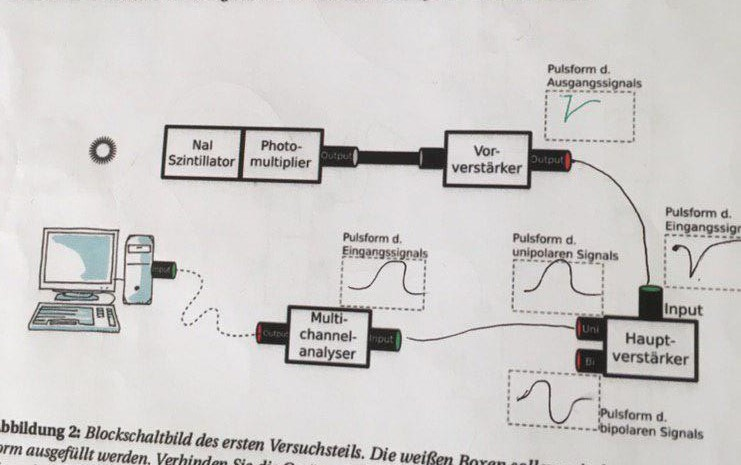
\includegraphics[scale=0.5]{Bilder/schaltung_energie}
	\caption[Schematischer Aufbau zur Energiemessung]{\small Der schematische Aufbau für die Messung der Energiespektren sowie die Signalformen der ein- und ausgehenden Signale sind hier eingezeichnet.}
	\label{schaltung_energie}
\end{figure}

\subsection{Koinzidenzmessung}
Zur Koinzidenzmessung wurden als Vorbereitung nach erster Untergrundmessung der Energiespektren die Ausgänge des Hauptverstärkers betrachtet. Hierbei wurde die Natrium Probe als Signalquelle gewählt, da diese auch bei der Koinzidenzmessung verwendet wird. Die uni- und bipolaren Signale unterscheiden sich hier aber kaum, was aus den Abbildungen \ref{uni_org} und \ref{bip_org} hervorgeht. Dies ist dennoch bei der eigentlichen Messung vernachlässigbar.\par
Am nächsten Tag wurde die Koinzidenzschaltung nach Abbildung \ref{schaltung_coinc}  aufgebaut. Es wird die Natrium Probe für alle weiteren Messungen verwendet. Die Energiefenster des SCA wurden mittels des MCA und des PC auf den $511\,$keV Vernichtungspeak des Natriumspektrums eingestellt. Anschließend wurden die Signale des SCA mit dem Oszilloskops aufgezeichnet. Diese sind in den Abbildungen \ref{SCA_pos} und \ref{SCA_neg} zu finden. Anschließend wurde das Ausgangssignal der Timing-Unit eingestellt und aufgezeichnet. Es sieht analog zum positiven Signal des SCA aus, nur ist das Plato negativ im Vergleich zur Nulllinie. Anschließend wurde die Verzögerung der Signale zueinander soweit angepasst, dass die Mehrheit der Signale überlappte. \par
Nun wurde mit der Koinzidenzmessung begonnen. Der organische Szintillator wurde in die $0^\circ$ Stellung gebracht um die Messzeit festzulegen. Es wurden 100s Gewählt, was zu einem relativen Fehler von $\approx 3\%$ ergab. Anschließend wurde von $0^\circ$ beginnend Messungen bei unterschiedlichen Winkeln in immer größer werdenden Schritten  durchgeführt. Als das erste mal $90^\circ$ erreicht wurde, ist eine Hintergrundmessung mit Messzeit $10^5\,$s durchgeführt worden. Anschließend wurde erneut von $0^\circ$ gestartet und in die andere Richtung gemessen. Hier wurde bei $90^\circ$ keine Untergrundmessung durchgeführt.

\begin{figure}[h]
	\centering
	\includegraphics[scale=0.5]{Bilder/pl_uni}
	\caption[Unipolares Signal des Organischen Amp.]{\small Im Bild ist das unipolare Signal des Hauptverstärker des organischen Szintillators zu sehen. Es ist Auffällig, dass sich unipolares und bipolares Signal dieses Verstärkers sehr ähneln.}
	\label{uni_org}
\end{figure}
\begin{figure}[h]
	\centering
	\includegraphics[scale=0.5]{Bilder/pl_bi}
	\caption[Bipolares Signal des Organischen Amp.]{\small Im Bild ist das unipolare Signal des Hauptverstärker des organischen Szintillators zu sehen. }
	\label{bip_org}
\end{figure}


\begin{figure}[h]
	\centering
	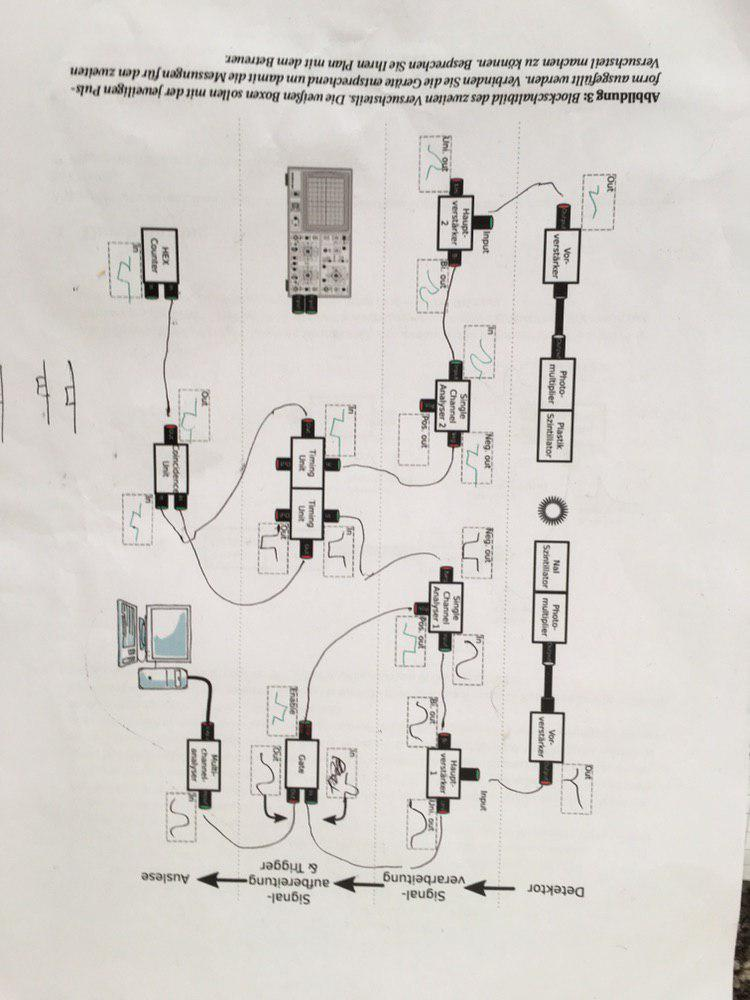
\includegraphics[scale=0.45,angle=90]{Bilder/schaltung_coinc}
	\caption[Schematischer Aufbau zur Koinzidenzmessung]{\small Der schematische Aufbau für die Koinzidenzmessung sowie die Signalformen der ein- und ausgehenden Signale sind hier eingezeichnet.}
	\label{schaltung_coinc}
\end{figure}

\begin{figure}[h]
	\centering
	\includegraphics[scale=0.5]{Bilder/sca_pos}
	\caption[Positives Signal des SCA]{\small Im Bild ist das positive Signal des SCA sichtbar. Die Signalform ist vergleichbar mit den sonstigen Rechtecksignalen.}
	\label{SCA_pos}
\end{figure}

\begin{figure}[h]
	\centering
	\includegraphics[scale=0.5]{Bilder/sca_neg}
	\caption[Negatives Signal des SCA]{\small Im Bild ist das negative Signal des SCA sichtbar.}
	\label{SCA_neg}
\end{figure}